\documentclass[UTF8,zihao=-4]{ctexart}
\usepackage[a4paper,margin=2.5cm]{geometry}
\usepackage{amsmath, amssymb, amsthm}
\usepackage{bm}
\usepackage{hyperref}
\usepackage{graphicx}
\usepackage{caption}
\usepackage{listings}
\usepackage{xcolor}
\usepackage{float}
\usepackage{placeins}
\graphicspath{{figures/}}

% Code style
\lstdefinestyle{code}{
  basicstyle=\ttfamily\small,
  numbers=left,
  numberstyle=\tiny,
  numbersep=8pt,
  keywordstyle=\color{blue},
  commentstyle=\color{teal!70!black},
  stringstyle=\color{orange!70!black},
  showstringspaces=false,
  breaklines=true,
  frame=single,
  framerule=0.3pt,
  rulecolor=\color{black!15}
}
\lstset{style=code}

\title{模型压缩与部署技术}
\author{}
\date{\today}

\begin{document}
\maketitle
\tableofcontents
\FloatBarrier

\section{模型剪枝、蒸馏与量化}
压缩技术以尽量保持精度的方式减少参数量、显存占用与推理时延。图~\ref{fig:compression_overview_cn} 对比了剪枝、蒸馏与量化的整体流程。

\subsection{剪枝}
剪枝通过二值掩码 $\mathbf{M}$ 让有效权重变为 $\tilde{\mathbf{W}} = \mathbf{M} \odot \mathbf{W}$:
\begin{itemize}
  \item \textbf{非结构化剪枝:} 对权重逐个置零(如迭代幅度剪枝、$l_0$ 正则)。需配合稀疏矩阵库才能获得运行时收益。
  \item \textbf{结构化剪枝:} 删除通道、卷积核或注意力头,满足硬件的稠密计算需求。可通过
  \begin{equation}
    \min_{\mathbf{M}} \mathcal{L}(\mathbf{M} \odot \mathbf{W}) + \lambda \|\mathbf{M}\|_0, \quad \text{s.t. } \sum_{c} M_c \le K
  \end{equation}
  控制保留的通道数量 $K$。
  \item \textbf{动态剪枝:} 根据输入自适应选择子网络(如 SkipNet、动态 token 剪枝),以强化代价与精度的实时权衡。
\end{itemize}
“彩票假说”表明经过恰当初始化的子网络可单独收敛到与原模型相当的精度。实际流程常在剪枝后接蒸馏或额外微调以恢复性能。

\subsection{知识蒸馏}
蒸馏将教师模型 $f_T$ 的知识迁移到学生模型 $f_S$。常见的软硬标签混合损失:
\begin{equation}
  \mathcal{L}_{\mathrm{KD}} = (1-\alpha)\,\mathcal{L}_{\mathrm{CE}}(f_S(\mathbf{x}), \mathbf{y}) + \alpha T^2 \mathrm{KL}\left(\sigma\left(\frac{f_T(\mathbf{x})}{T}\right) \,\Big\|\, \sigma\left(\frac{f_S(\mathbf{x})}{T}\right)\right),
\end{equation}
其中 $T$ 为温度,$\alpha$ 为蒸馏权重。变体包括中间特征对齐、注意力图迁移、自蒸馏(同一模型多阶段蒸馏)等。

\subsection{量化}
量化通过缩放因子 $s$ 与零点 $z$ 将浮点数映射到低比特表示:
\begin{equation}
  q = \mathrm{clip}\left(\mathrm{round}\left(\frac{x}{s}\right) + z, q_{\min}, q_{\max}\right).
\end{equation}
主要类型为:
\begin{itemize}
  \item \textbf{训练后量化(PTQ):} 仅需少量校准数据即可导出 INT8;适用于容忍少量精度损失的场景。
  \item \textbf{量化感知训练(QAT):} 在训练期间模拟量化(使用 STE),可在 INT8 乃至 INT4 仍保持高精度。
  \item \textbf{混合精度量化:} 按层分配不同比特位,借助整数规划或强化学习满足精度/延迟双指标。
\end{itemize}
针对 Transformer 的 SmoothQuant 通过权重与激活的缩放重分配抑制激活异常值,从而提升 INT8 推理稳定性。

\subsection{流程整合}
实际工程常将剪枝、蒸馏与量化串联:先对教师模型剪枝,再蒸馏至小模型,最后进行量化感知微调。硬件感知的 NAS 则直接搜索易量化的架构。下面展示一段联合流程的伪代码:

\begin{lstlisting}[language=Python, caption={剪枝 + 蒸馏 + 量化感知训练联合流程示例。}]
teacher = load_pretrained_model()
student = initialize_compact_model()

# 教师模型结构化剪枝
for step in range(prune_steps):
    loss = training_step(teacher, data_batch)
    loss.backward()
    apply_structured_pruning(teacher, sparsity_schedule(step))

# 蒸馏训练学生模型
for epoch in range(kd_epochs):
    for batch in dataloader:
        teacher_logits = teacher(batch.inputs).detach()
        loss = kd_loss(student(batch.inputs), batch.labels, teacher_logits,
                       alpha=0.7, temperature=4.0)
        loss.backward()
        optimizer.step()
        optimizer.zero_grad()

# 量化感知微调
quantizer = prepare_qat(student, bitwidth=8)
for epoch in range(qat_epochs):
    for batch in dataloader:
        output = quantizer(batch.inputs)
        loss = criterion(output, batch.labels)
        loss.backward()
        optimizer.step()
        optimizer.zero_grad()
export_int8(quantizer, path="student_int8.onnx")
\end{lstlisting}

\begin{figure}[H]
  \centering
  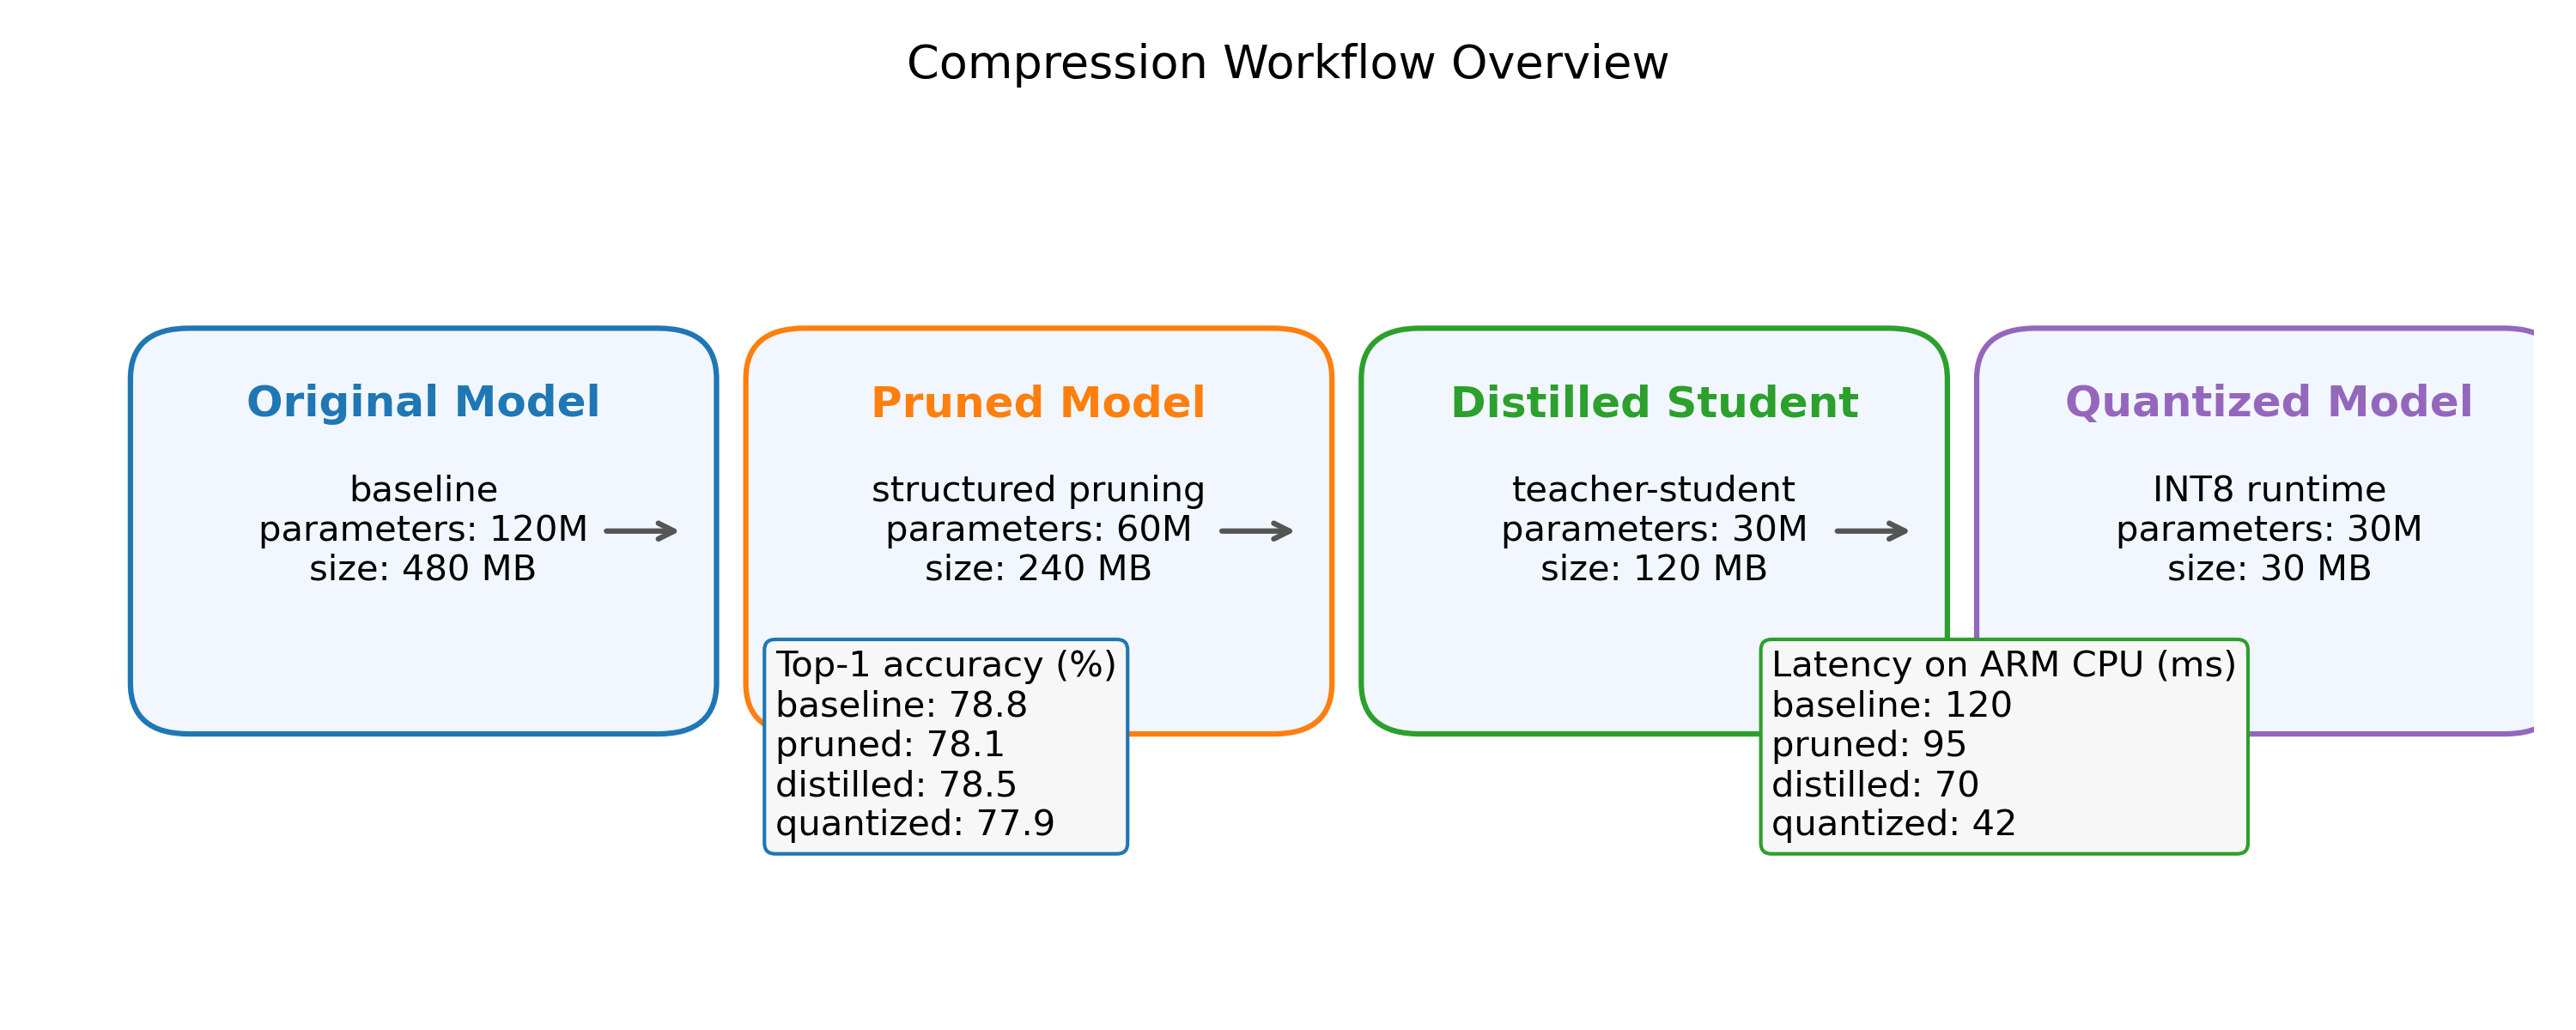
\includegraphics[width=0.9\textwidth]{compression_overview.png}
  \caption{剪枝、蒸馏、量化流程及其精度-模型大小折衷。}
  \label{fig:compression_overview_cn}
\end{figure}
\FloatBarrier

\section{部署到移动端/边缘设备(TensorRT, ONNX, TFLite)}
边缘部署需要将训练好的模型转换成适配目标硬件的运行时。图~\ref{fig:deployment_toolchain_cn} 总结了主要生态链路。

\subsection{ONNX 中间表示}
ONNX 以算子集(opset)的形式定义中间表示。将 PyTorch/TensorFlow 模型导出为 ONNX 图 $\text{Graph} = (\mathcal{V}, \mathcal{E}, \mathcal{O})$ 后,可在不同推理引擎之间交换。需注意导出端与推理端的 opset 版本一致,同时执行常量折叠、形状推断以减小模型。

\subsection{TensorRT 优化}
TensorRT 接收 ONNX 输入并编译为 CUDA 引擎,核心优化包括层融合、精度校准(FP16/INT8)与内核自动调优。动态形状模型需要在构建期指定优化 profile 的最小/最大/最优尺寸。ONNX Runtime 可通过 TensorRT Execution Provider 优先执行已支持的算子,回退到 GPU/CPU 上实现兼容。

\subsection{TensorFlow Lite(TFLite)}
TFLite 将 SavedModel 转换为紧凑的 flatbuffer,内置面向移动 CPU、GPU 与 NPU 的算子。量化感知训练导出的 INT8 模型可直接部署到 Edge TPU。Delegate 机制(NNAPI、Core ML 等)可将特定算子 offload 到厂商加速器。

\subsection{部署清单}
\begin{itemize}
  \item 验证导出模型与原框架之间的数值一致性。
  \item 在真实并发与输入分布下测试内存占用与延迟。
  \item 为不支持的算子准备回退路径或自定义插件。
  \item 监控算子覆盖率与精度,必要时做图重写或算子替换。
\end{itemize}
下面示例演示 PyTorch 导出 ONNX 并使用 TensorRT Python API 构建引擎:

\begin{lstlisting}[language=Python, caption={PyTorch 导出 ONNX 并构建 TensorRT 引擎示例。}]
import torch
import onnx
import tensorrt as trt

model = build_model().eval().cuda()
dummy = torch.randn(1, 3, 224, 224, device="cuda")
torch.onnx.export(model, dummy, "model.onnx",
                  input_names=["input"], output_names=["logits"],
                  opset_version=17, do_constant_folding=True,
                  dynamic_axes={"input": {0: "batch"}, "logits": {0: "batch"}})

onnx_model = onnx.load("model.onnx")
onnx.checker.check_model(onnx_model)

logger = trt.Logger(trt.Logger.INFO)
builder = trt.Builder(logger)
network = builder.create_network(1 << int(trt.NetworkDefinitionCreationFlag.EXPLICIT_BATCH))
parser = trt.OnnxParser(network, logger)
with open("model.onnx", "rb") as f:
    parser.parse(f.read())

config = builder.create_builder_config()
config.set_memory_pool_limit(trt.MemoryPoolType.WORKSPACE, 1 << 30)
if builder.platform_has_fast_int8:
    config.set_flag(trt.BuilderFlag.INT8)
    config.int8_calibrator = gather_calibration_data()

engine = builder.build_engine(network, config)
with open("model.plan", "wb") as f:
    f.write(engine.serialize())
\end{lstlisting}

\begin{figure}[H]
  \centering
  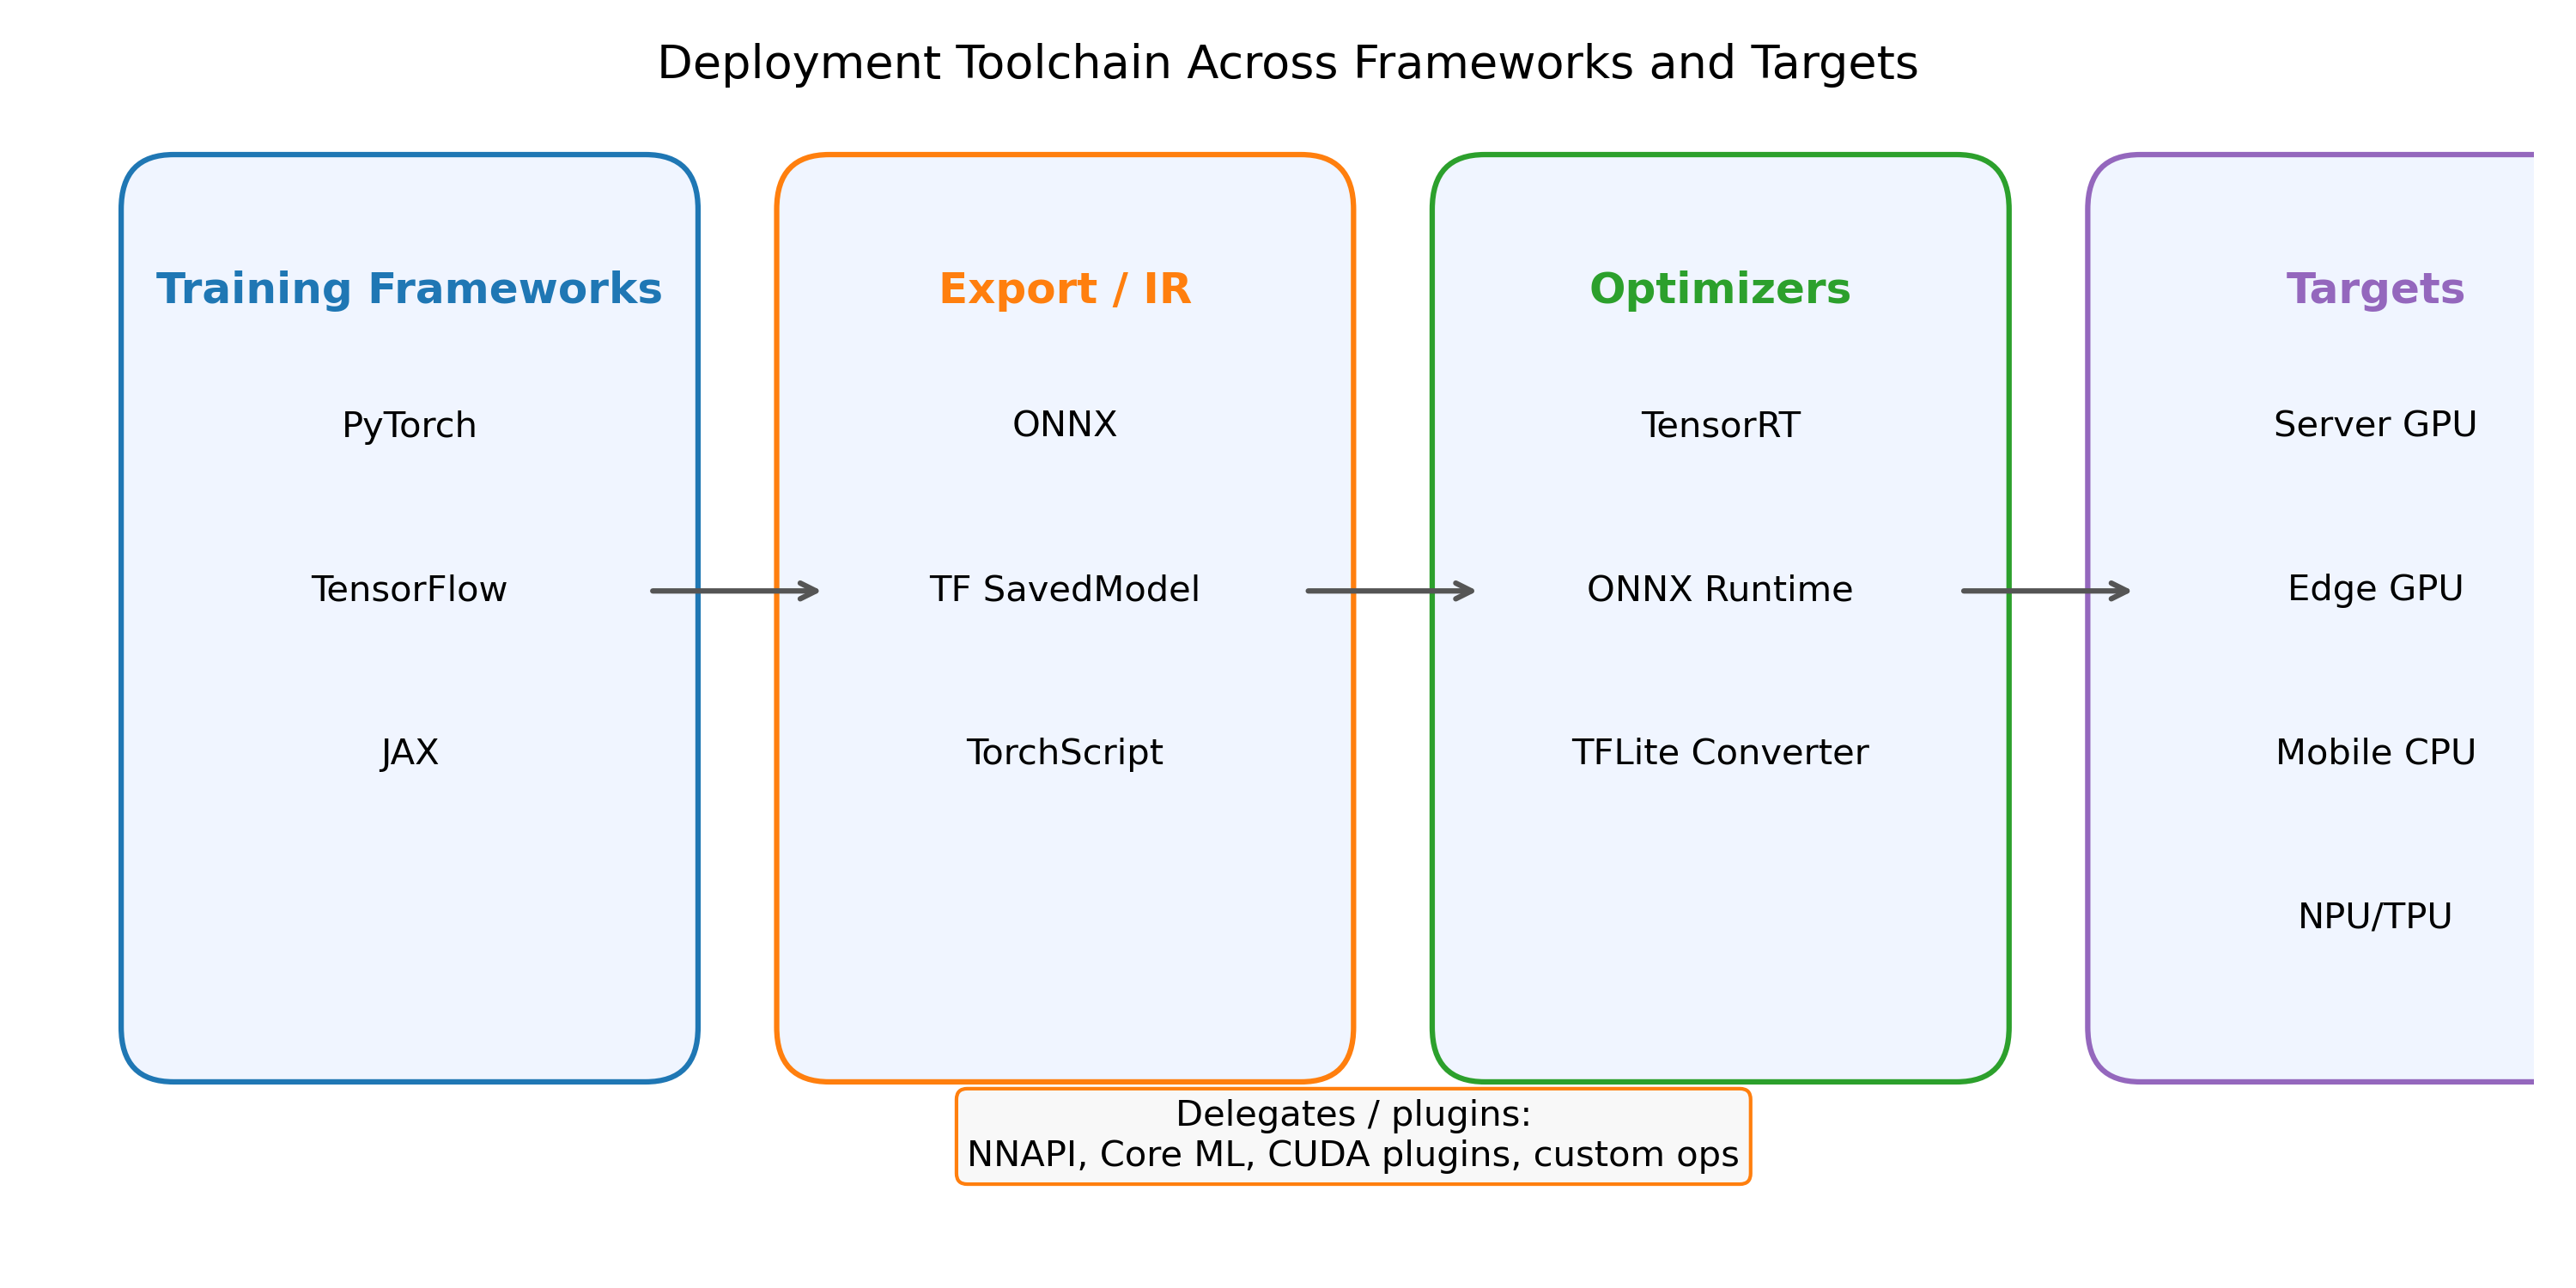
\includegraphics[width=0.9\textwidth]{deployment_toolchain.png}
  \caption{ONNX、TensorRT、TFLite 等部署链路及可选 delegate。}
  \label{fig:deployment_toolchain_cn}
\end{figure}
\FloatBarrier

\section{推理加速}
推理优化的目标是降低延迟、提升吞吐与能效。图~\ref{fig:latency_breakdown_cn} 展示了推理延迟分解,而图~\ref{fig:accelerated_inference_strategies_cn} 总结了多层面的加速手段。

\subsection{算子与图优化}
算子融合(Conv-BN-ReLU)减少访存;图编译器(TVM、XLA、TorchInductor)通过循环分块、向量化、布局重排减少计算与内存开销。延迟可近似为
\begin{equation}
  L = \sum_{i=1}^{N} \left(\frac{C_i}{\mathrm{FLOP/s}} + \frac{M_i}{\mathrm{BW}}\right),
\end{equation}
调度策略旨在同时降低计算 $C_i$ 与内存流量 $M_i$。

\subsection{批处理与服务编排}
批处理摊平请求开销。在线服务到达率为 $\lambda$、服务率为 $\mu$ 时,排队延迟可用 Erlang C 模型估计。动态批处理(如 Triton Inference Server)在延迟预算内聚合请求;自回归模型则可通过推测解码、流水化 beam search 缩短单 token 延迟。

\subsection{硬件加速}
专用加速器(Edge TPU、Tensor Core)支持低精度矩阵运算。内存受限模型依赖 HBM 与稀疏友好硬件。移动端可借助 CPU 向量引擎(NEON、AVX512)以及 XNNPACK、oneDNN 等库。

\subsection{监控与 A/B 实验}
线上环境需持续监控延迟分位数(P50/P95/P99)、吞吐与功耗。通过金丝雀发布、特性开关逐步替换新模型,确保性能提升同时避免负面影响。

\begin{lstlisting}[language=Python, caption={Triton Inference Server 动态批处理配置示例。}]
name: "resnet_triton"
platform: "tensorrt_plan"
max_batch_size: 32
input [
  { name: "input", data_type: TYPE_FP16, dims: [3, 224, 224] }
]
output [
  { name: "logits", data_type: TYPE_FP16, dims: [1000] }
]
dynamic_batching {
  preferred_batch_size: [4, 8, 16, 32]
  max_queue_delay_microseconds: 2000
}
instance_group [
  { kind: KIND_GPU, count: 2, gpus: [0, 1] }
]
\end{lstlisting}

\begin{figure}[H]
  \centering
  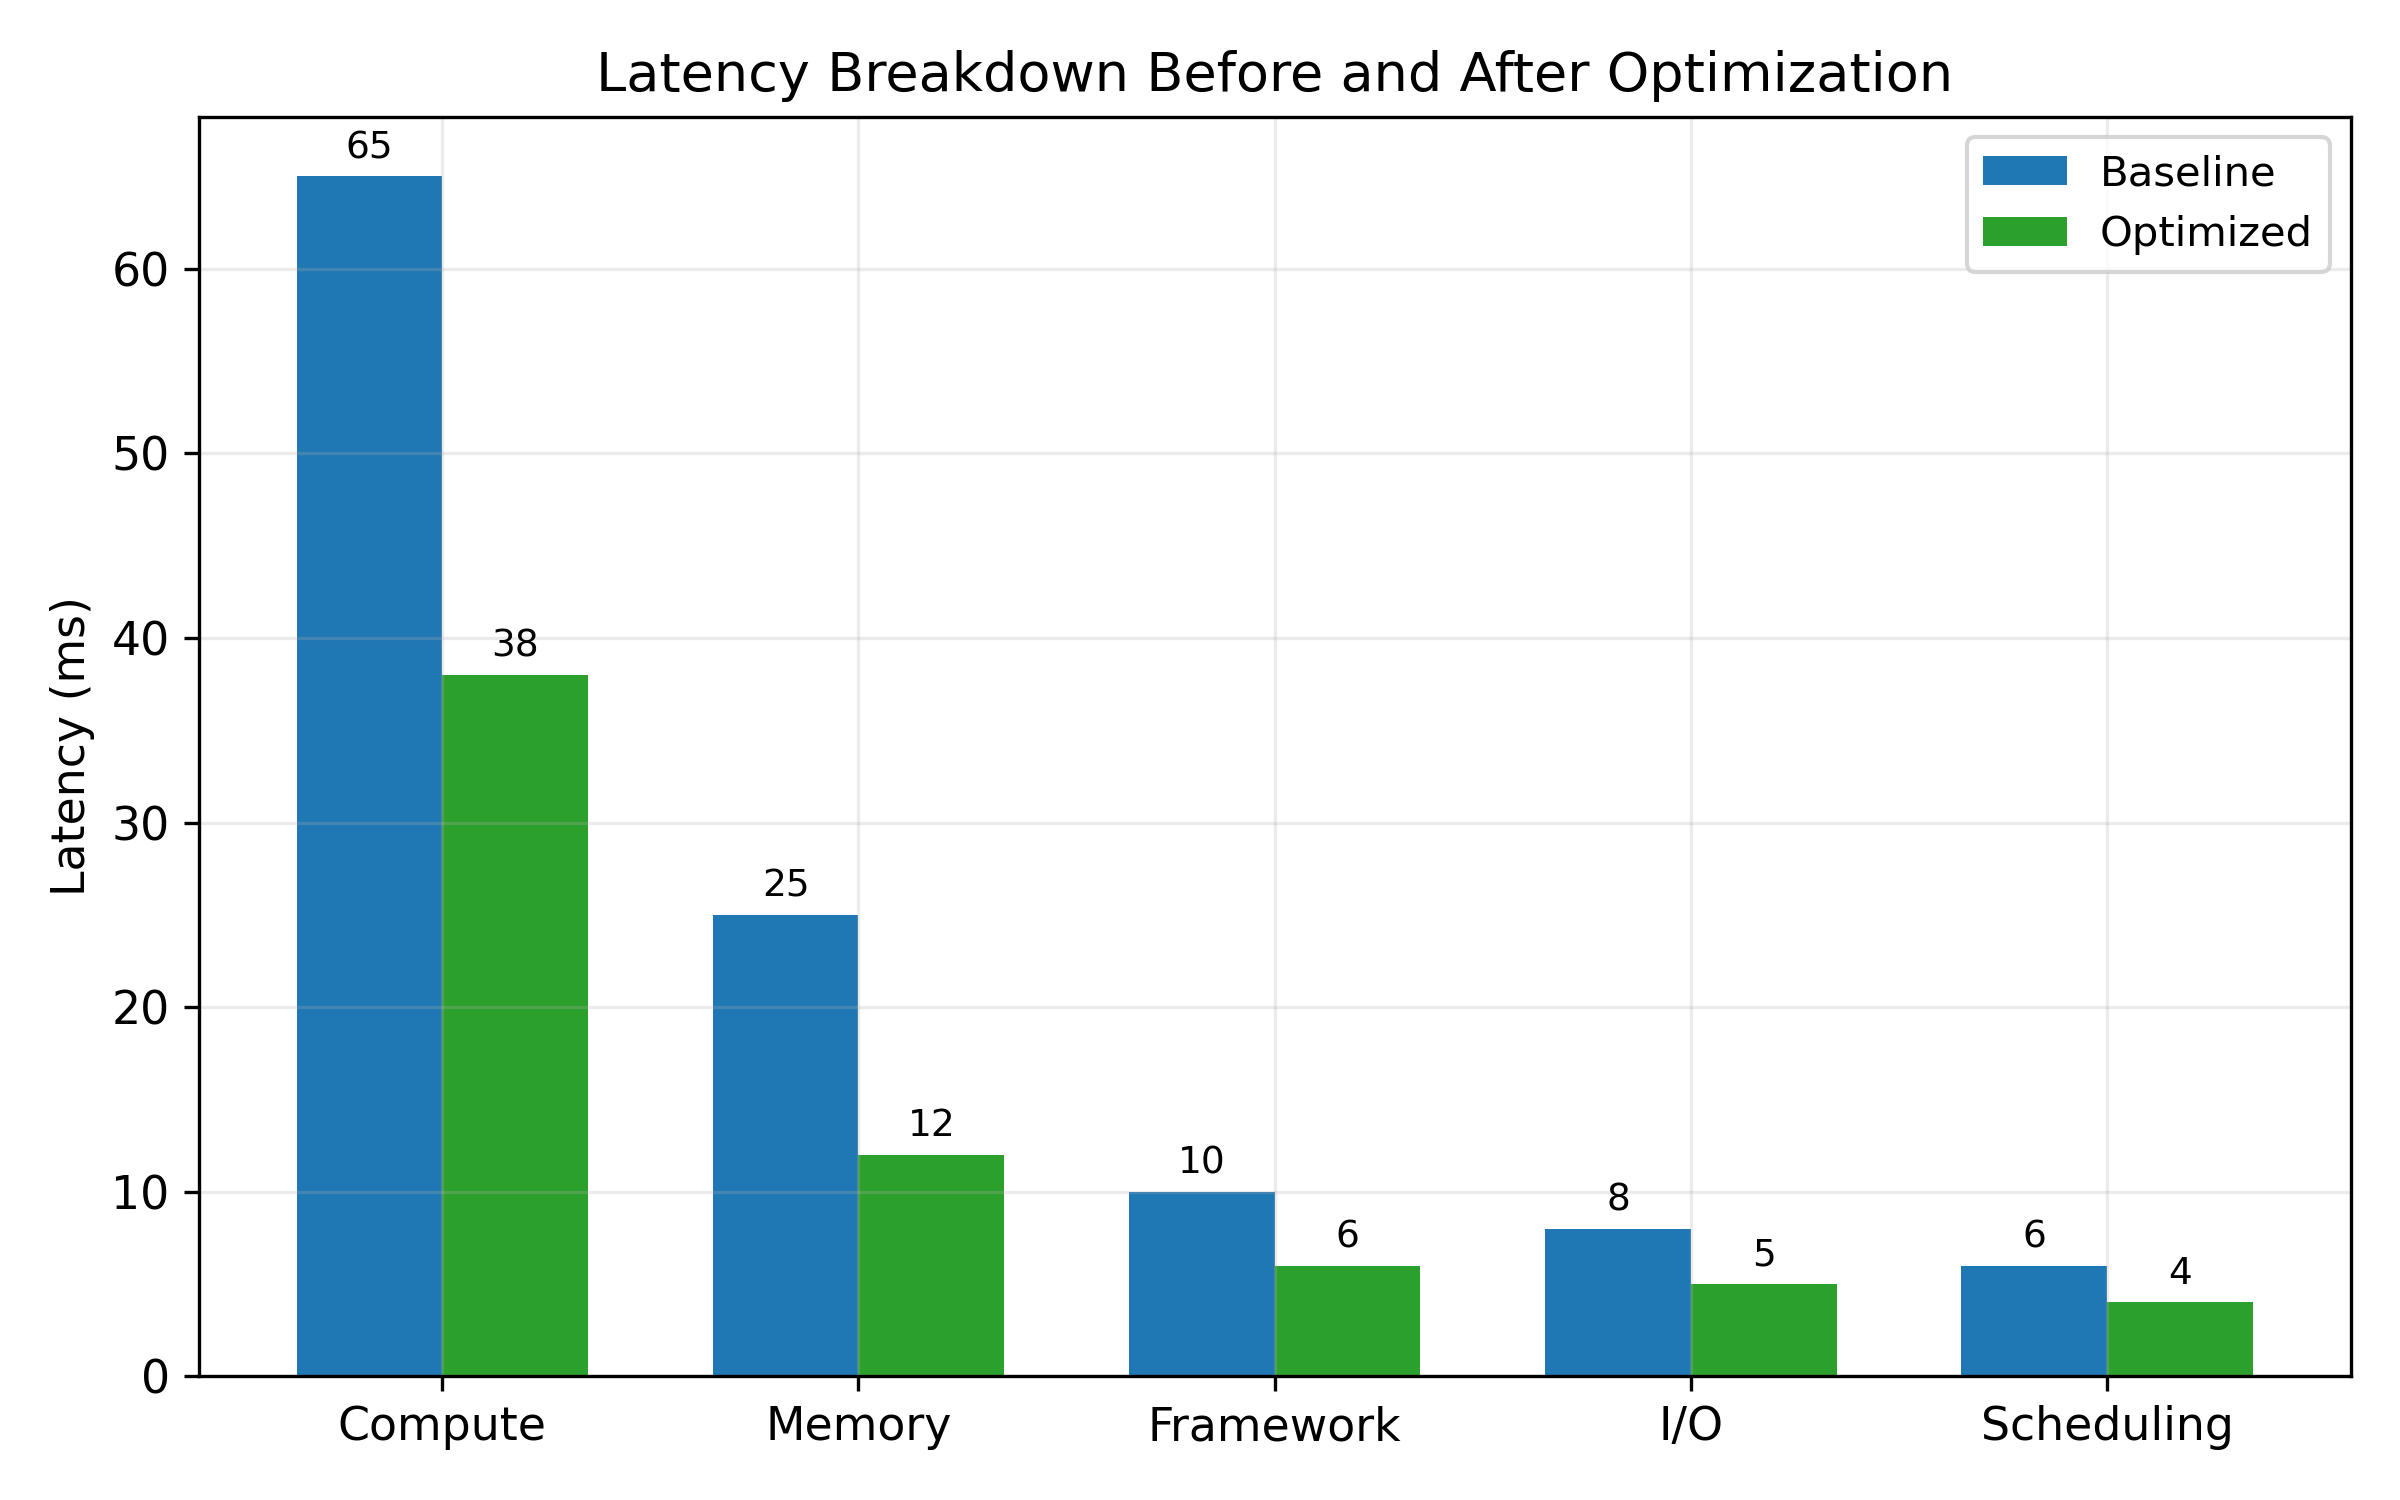
\includegraphics[width=0.85\textwidth]{latency_breakdown.png}
  \caption{推理延迟各组成部分的分析。}
  \label{fig:latency_breakdown_cn}
\end{figure}

\begin{figure}[H]
  \centering
  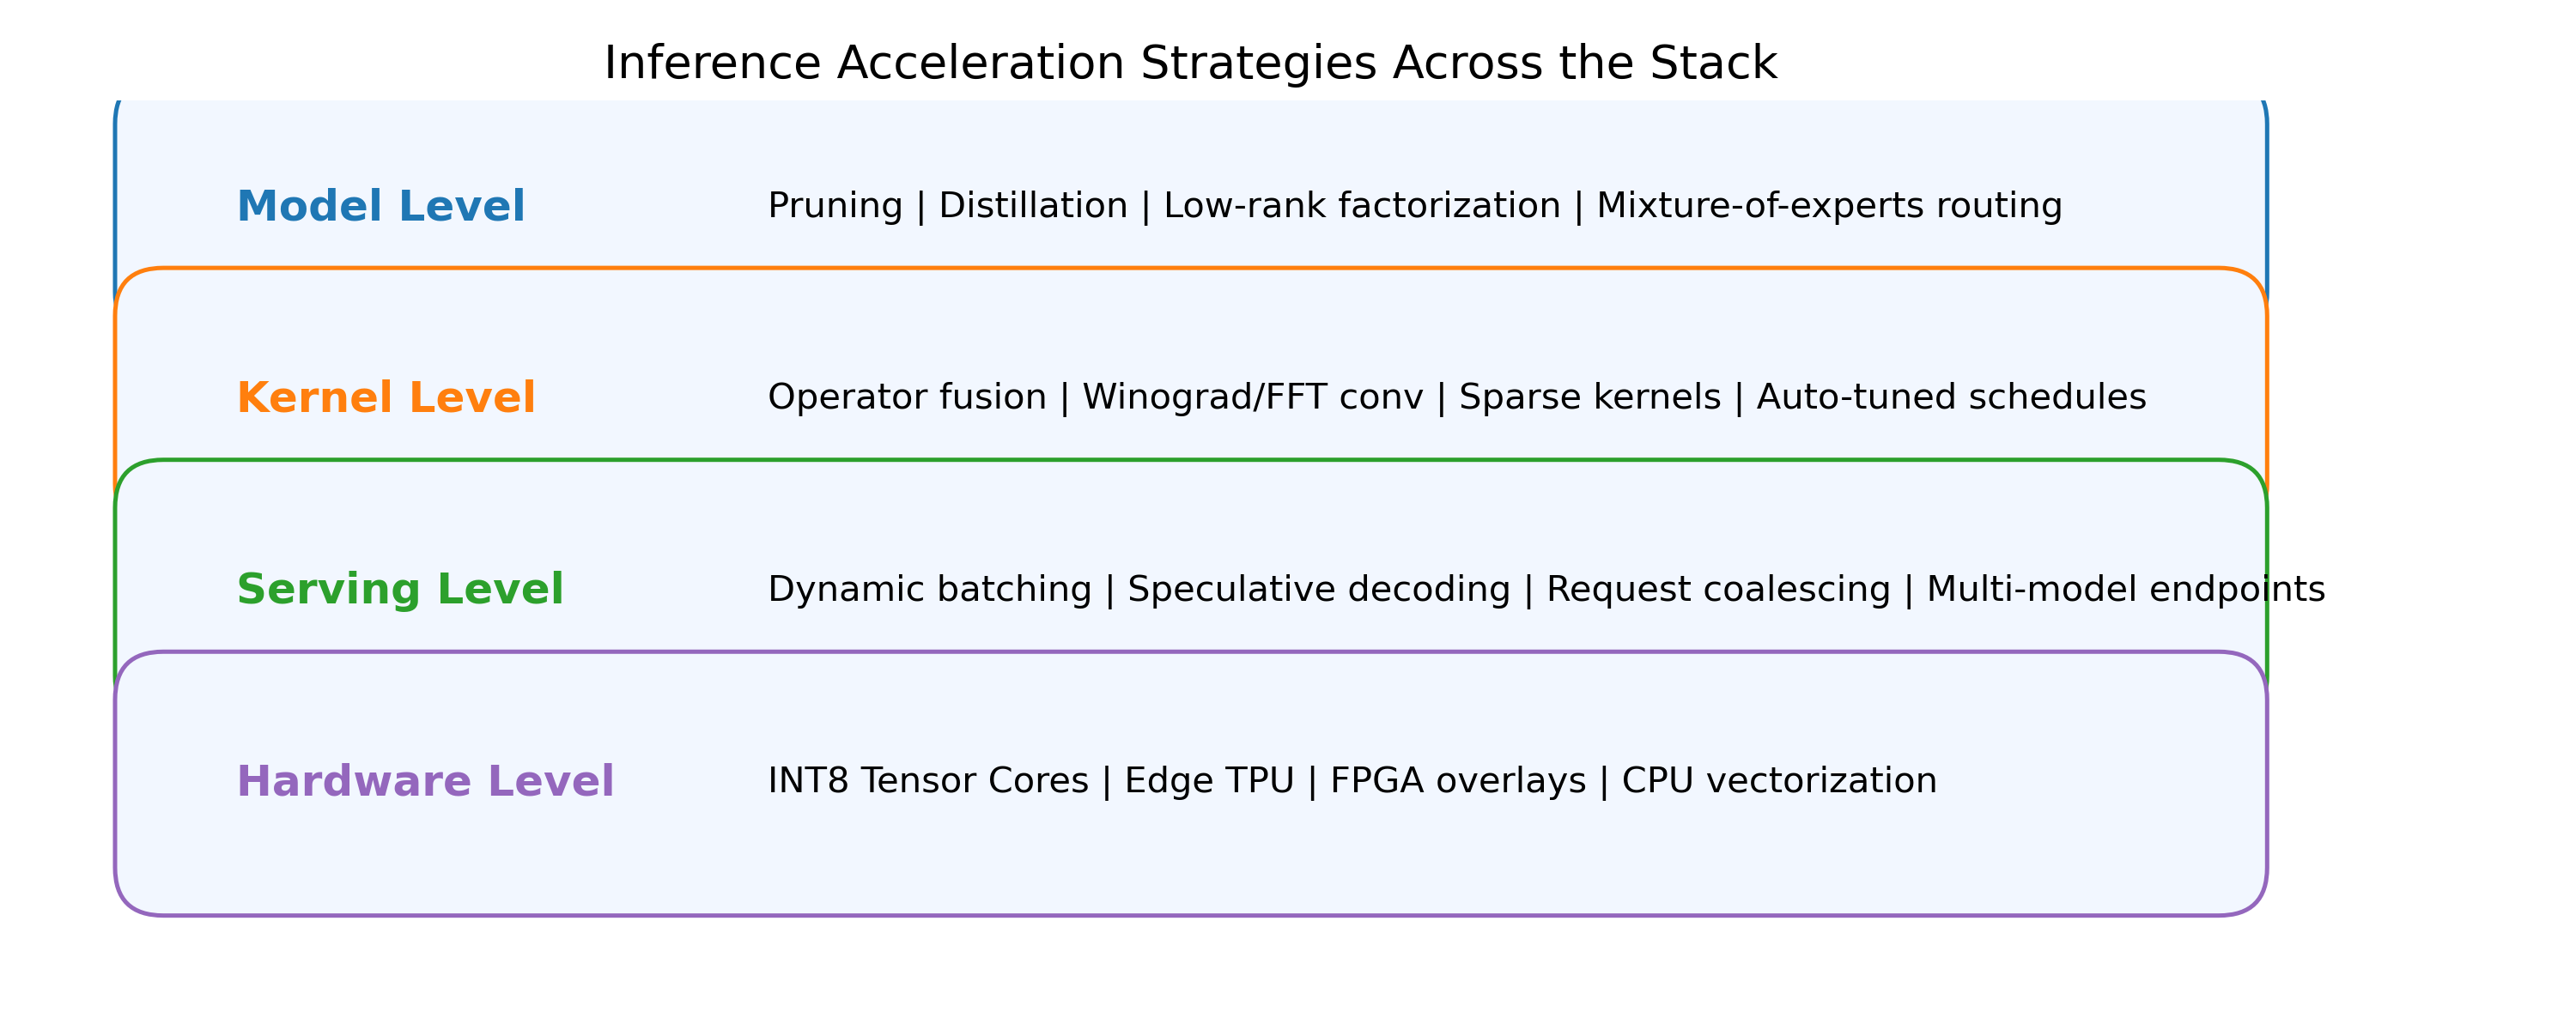
\includegraphics[width=0.9\textwidth]{accelerated_inference_strategies.png}
  \caption{模型、算子、服务、硬件多层面的推理加速策略。}
  \label{fig:accelerated_inference_strategies_cn}
\end{figure}
\FloatBarrier

\section*{延伸阅读}
\begin{itemize}
  \item Song Han 等:《Learning both Weights and Connections for Efficient Neural Networks》,NIPS 2015。
  \item Geoffrey Hinton 等:《Distilling the Knowledge in a Neural Network》,NIPS 2015 Workshop。
  \item Jacob 等:《Quantization and Training of Neural Networks for Efficient Integer-Arithmetic-Only Inference》,CVPR 2018。
  \item NVIDIA:《TensorRT Developer Guide》,2023。
  \item Jared Casper 等:《Amazon SageMaker Inference Recommender》,2022。
\end{itemize}

\end{document}
